%%%% BLOQUE DE DATOS %%%

\newcommand{\Title}{
	Guía de Usuario para Report
} %Titulo del reporte

\newcommand{\LogoUniversity}{img/logo.jpg} %logo de la universidad
\newcommand{\NameUniversity}{Universidad Galileo} %Nombre de la universidad
\newcommand{\Date}{
	Guatemala, 6 de marzo de 2020
} %Fecha de entrega
\newcommand{\Faculty}{Facultad FISICC} %Nombre de la facultad
\newcommand{\Course}{
	Curso: *******
} %Nombre del curso
\newcommand{\ID}{
	Carnet: **** ****
}
\newcommand{\Student}{
	Alumno: Josué Benyamin Isaí Galeano Morales
} %Nombre del estudiante
\newcommand{\Section}{
	Secci\'on: *
} %Sección del estudiante
\newcommand{\Schedule}{
	Horario de laboratorio: 18:00 a 19:00
} %Horario
\newcommand{\Assistant}{
	Auxiliar: *******
} %Persona encargada
\newcommand{\Day}{
	Día de laboratorio: viernes
} %Dia en que recibe
%% FIN BLOQUE DE DATOS%%


%% NO ES NECESARIO MODIFICAR ESTA PARTE %%
\def\arraystretch{1.2}
\textbf{
	\small
	\hspace{-1 cm}
	\begin{minipage}{0.15\textwidth}
		%%%%%%%%%%%%%%%%% LOGO %%%%%%%%%%%%%%%%%%%%%%%%%%%%%%%
		\includegraphics[scale=0.5]{\LogoUniversity}
	\end{minipage}
	\begin{minipage}{0.7\textwidth}
		\resizebox{1.25\textwidth}{!}{
			\begin{tabular}{ll}
				\hline 
				%%%%% PARTE SUPERIOR DE LA TABLA DE DATOS %%%%%%%%%%%%%%%%%%%%%%%
				\NameUniversity & \Date \\
				\hline
				\rowcolor{lightgray}
				\Faculty & \Student\\
				\hline 
				\Course & \ID\\
				\hline\rowcolor{lightgray}
				\Section & \Schedule\\
				\hline 
				\Assistant & \Day\\
				\hline
			\end{tabular}
		}
	\end{minipage}
}

\vspace{0.5cm}
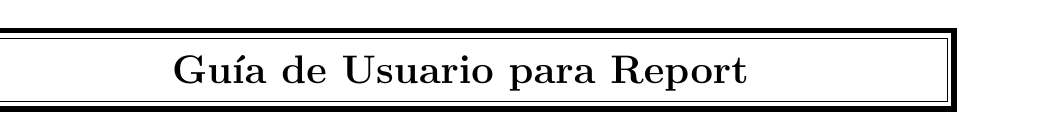
\begin{tikzpicture}
\hspace{-1 cm}
\draw (0.1,0.1) rectangle (1.043\textwidth,0.9);
\draw[line width=0.7mm] (0,0) rectangle (1.05\textwidth,1);
\node[font=\Large] at (0.525\textwidth, 0.45) {\textbf{\Title}};
\end{tikzpicture}		

\def\arraystretch{1}

\vspace*{0.5 cm}
